\documentclass[letterpaper,fleqn]{article}

\usepackage{enumerate}
\usepackage{amsmath}
\usepackage{mathtools}
\usepackage{blkarray}
%\usepackage{amssymb}
\usepackage[letterpaper, margin=1in]{geometry}
\usepackage{tikz}

\begin{document}
	\begin{enumerate}
		\item [\textbf{2.1}] \quad
		\begin{enumerate}
			\item [2.] 
			$\textbf{A}=\begin{bmatrix}
				E & R & S & T & A \\
				N & P & O & C & W \\
				H & B & U & I & L \\
				M & G & Y & F & K \\
			\end{bmatrix}$
			\begin{enumerate}[(a)]
				\item
				$a_{31}$, $a_{11}$, $a_{35}$, $a_{22}$ \\
				HELU
				
				\item
				$a_{35}$, $a_{34}$, $a_{21}$, $a_{11}$, $a_{15}$, $a_{15}$ \\
				LINEAR
				
				\item
				$a_{11}$, $a_{35}$, $a_{32}$, $a_{23}$, $a_{25}$ \\
				ELBOW 
				
				\item
				$a_{25}$, $a_{15}$, $a_{14}$, $a_{24}$, $a_{31}$, $a_{23}$, $a_{33}$, $a_{14}$ \\
				WATCHOUT
			\end{enumerate} 
									
			\item [12.]
			$\textbf{A}=\begin{bmatrix}
				1 & 2 & 3 & 4 \\
				2 & 4 & 6 & 8 \\
				3 & 5 & 7 & 9 \\
			\end{bmatrix}$ and $\textbf{B}=\begin{bmatrix*}[r]
				-1 & 0 & 2 & 1 \\
				2 & -1 & -1 & 0 \\
				2 & 0 & 0 & 2 \\
			\end{bmatrix*}$
			\begin{enumerate}
				\item [(b)]
				$2\textbf{B}=\begin{bmatrix*}[r]
					-2 & 0 & 4 & 2 \\
					4 & -2 & -2 & 0 \\
					4 & 0 & 0 & 4 \\
				\end{bmatrix*}$
				
				\item [(d)]
				$\textbf{A}+\textbf{B}=\begin{bmatrix*}
					0 & 2 & 5 & 5 \\
					4 & 3 & 5 & 8 \\
					5 & 5 & 7 & 11 \\
				\end{bmatrix*}$
			\end{enumerate}
		\end{enumerate}
		
		\item [\textbf{2.2}] \quad
		\begin{enumerate}
			\item [10.]
			\begin{alignat*}{13}
				2x_1 & {}+{} & 3x_2 & {}-{} & 2x_3 & {}={} 
				& 5y_1 & {}+{} & 2y_2 & {}-{} & 3y_3 & {}+{} & 200 \\
				 x_1 & {}+{} & 4x_2 & {}+{} & 3x_3 & {}={} 
				& 6y_1 & {}-{} & 4y_2 & {}+{} & 4y_3 & {}-{} & 120 \\
				5x_1 & {}+{} & 2x_2 & {}-{} &  x_3 
				& {}={} & 2y_1 & {} {} &      & {}-{} & 2y_3 & {}+{} & 350
			\end{alignat*}
			\begin{enumerate}[(a)]
				\item 
				$\textbf{A}=\begin{bmatrix*}[r]
					2 & 3 & -2 \\
					1 & 4 & 3 \\
					5 & 2 & -1 \\
				\end{bmatrix*}$, $\textbf{x}=\begin{bmatrix*}
					x_1 \\
					x_2 \\
					x_3 \\
				\end{bmatrix*}$ \\
				$\textbf{B}=\begin{bmatrix*}[r]
					5 & 2 & -3 & 200 \\
					6 & -4 & 4 & -120 \\
					2 & 0 & -2 & 350 \\
				\end{bmatrix*}$, $\textbf{y}=\begin{bmatrix*}
					y_1 \\
					y_2 \\
					y_3 \\
					1 \\
				\end{bmatrix*}$ \\
				$\textbf{Ax}=\textbf{By}$
				
				\item
				$\textbf{A}=\begin{bmatrix*}[r]
					2 & 3 & -2 & -5 & -2 & 3 \\
					1 & 4 & 3 & -6 & 4 & -4 \\
					5 & 2 & -1 & -2 & 0 & 2 \\
				\end{bmatrix*}$, $\textbf{n}=\begin{bmatrix*}
					x_1 \\
					x_2 \\
					x_3 \\
					y_1 \\
					y_2 \\
					y_3 \\
				\end{bmatrix*}$, $\textbf{b}=\begin{bmatrix*}[r]
					200 \\
					-120 \\
					350 \\
				\end{bmatrix*}$ \\
				$\textbf{An}=\textbf{b}$ \\
			\end{enumerate}
			
			\item [18.]
			$\textbf{A}=\begin{bmatrix*}
				1 & 2 & 3 & 4 \\
				2 & 4 & 6 & 8 \\
				3 & 6 & 7 & 9 \\
			\end{bmatrix*}$, $\textbf{B}=\begin{bmatrix*}[r]
				1 & 0 & -1 \\
				2 & -2 & 0 \\
				0 & 1 & -1 \\
			\end{bmatrix*}$, $\textbf{C}=\begin{bmatrix*}
				5 & 4 & 1 \\
				1 & 0 & 2 \\
				3 & 2 & 1 \\
				0 & 1 & 3 \\
			\end{bmatrix*}$
			\begin{enumerate}[(a)]
				\item \textbf{AB} does not exist.
				
				\item $\textbf{BA}=\begin{bmatrix*}[r]
					-2 & -4 & -4 & -5 \\
					-2 & -4 & -6 & -8 \\
					-1 & -2 & -1 & -1 \\
				\end{bmatrix*}$
				
				\item $\textbf{AC}=\begin{bmatrix*}[r]
					16 & 14 & 20 \\
					32 & 28 & 40 \\
					42 & 35 & 49 \\
				\end{bmatrix*}$
				
				\item $\textbf{CA}=\begin{bmatrix*}[r]
					16 & 32 & 46 & 61 \\
					7 & 14 & 17 & 22 \\
					10 & 20 & 28 & 37 \\
					11 & 22 & 27 & 35 \\
				\end{bmatrix*}$
				
				\item $\textbf{CB}=\begin{bmatrix*}[r]
					13 & -7 & -6 \\
					1 & 2 & -3 \\
					7 & -3 & -4 \\
					2 & 1 & -3 \\
				\end{bmatrix*}$
			\end{enumerate}
			
			
			
			\item [22.]
			$\begin{blockarray}{ccc}
				& \text{Store $A$} & \text{Store $B$} \\
				\begin{block}{l[cc]}
					\text{Apple} & .10 & .15  \\
					\text{Orange} & .15 & .20  \\
					\text{Pear} & .10 & .10  \\
				\end{block}
			\end{blockarray}$
			$\begin{blockarray}{cccc}
				& \text{Apple} & \text{Orange} & \text{Pear} \\
				\begin{block}{l[ccc]}
					\text{Person $A$} & 5 & 10 & 3  \\
					\text{Person $B$} & 4 & 5 & 5  \\
				\end{block}
			\end{blockarray}$ \\
			$\begin{blockarray}{ccc}
				& \text{Person $A$} & \text{Person $B$} \\
				\begin{block}{l[cc]}
					\text{Town 2} & 1000 & 500\\
					\text{Town 1} & 2000 & 1000 \\
				\end{block}
			\end{blockarray}$
			\begin{enumerate}[(a)]
				\item
				$\begin{bmatrix*}
					5 & 10 & 3 \\
					4 & 5 & 5 \\
				\end{bmatrix*}
				\begin{bmatrix*}
					.10 & .15 \\
					.15 & .20 \\
					.10 & .10 \\
				\end{bmatrix*}
				=
				\begin{blockarray}{ccc}
					& \text{Store $A$} & \text{Store $B$} \\
					\begin{block}{l[cc]}
						\text{Person $A$} & 2.30 & 3.05 \\
						\text{Person $B$} & 1.65 & 2.10 \\
					\end{block}
				\end{blockarray}$
				
				\item
				$\begin{bmatrix*}
					1000 & 500 \\
					2000 & 1000 \\
				\end{bmatrix*}
				\begin{bmatrix*}
					5 & 10 & 3 \\
					4 & 5 & 5 \\
				\end{bmatrix*}
				=
				\begin{blockarray}{cccc}
					& \text{Apple} & \text{Orange} & \text{Pear} \\
					\begin{block}{c[ccc]}
						\text{Town 1} & 7000 & 12500 & 5500 \\
						\text{Town 2} & 14000 & 25000 & 11000 \\
					\end{block}
				\end{blockarray}$
				
				\item
				$\begin{bmatrix*}
					7000 & 12500 & 5500 \\
					14000 & 25000 & 11000 \\
				\end{bmatrix*}
				\begin{bmatrix*}
					.10 & .15 \\
					.15 & .20 \\
					.10 & .10 \\
				\end{bmatrix*}
				=
				\begin{blockarray}{ccc}
					& \text{Store $A$} & \text{Store $B$} \\
					\begin{block}{c[cc]}
						\text{Town 1} & 3125 & 4100 \\
						\text{Town 2} & 6250 & 8200 \\
					\end{block}
				\end{blockarray}$
			\end{enumerate}
		\end{enumerate}
		
		\item [\textbf{2.3}] \quad
		\begin{enumerate}
			\item [1.] \quad
			\begin{enumerate}
				\item [(c)]
				$\begin{bmatrix*}
					0 & 0 & 1 & 1 & 0 & 0 \\
					0 & 1 & 1 & 0 & 1 & 1 \\
					1 & 1 & 0 & 0 & 0 & 1 \\
					1 & 0 & 0 & 1 & 1 & 1 \\
					0 & 1 & 0 & 1 & 0 & 0 \\
					0 & 1 & 1 & 1 & 0 & 1 \\
				\end{bmatrix*}$ \\
				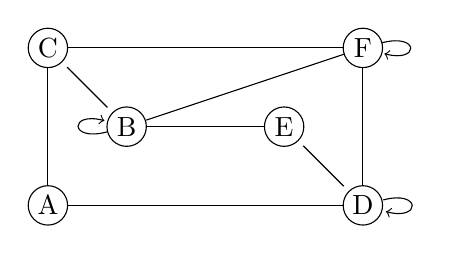
\begin{tikzpicture}
					\draw
					(0,0) circle (0.25) node[black] (a) {A}
					(1,1) circle (0.25) node[black] (b) {B}
					(0,2) circle (0.25) node[black] (c) {C}
					(4,0) circle (0.25) node[black] (d) {D}
					(3,1) circle (0.25) node[black] (e) {E}
					(4,2) circle (0.25) node[black] (f) {F}
					;
					\path (a) edge (c);
					\path (a) edge (d);
					\path (b) edge [loop left] (b);
					\path (b) edge (c);
					\path (b) edge (e);
					\path (b) edge (f);
					\path (c) edge (f);
					\path (d) edge [loop right] (d);
					\path (d) edge (e);
					\path (d) edge (f);
					\path (f) edge [loop right] (f);
				\end{tikzpicture}
			\end{enumerate}
			
			\item [2.] \quad
			\begin{enumerate}
				\item [(e)]
				$\begin{bmatrix*}
					0 & 1 & 1 & 1 & 1 & 1 \\
					1 & 0 & 1 & 1 & 0 & 0 \\
					1 & 1 & 0 & 1 & 0 & 0 \\
					1 & 1 & 1 & 0 & 0 & 0 \\
					1 & 0 & 0 & 0 & 0 & 0 \\
					1 & 0 & 0 & 0 & 0 & 0 \\
				\end{bmatrix*}$
			\end{enumerate}
			
			\item [3.] \quad
			\begin{enumerate}
				\item [(e)]
				${G_5}^2=\begin{bmatrix*}
					5 & 2 & 2 & 2 & 0 & 0 \\
					2 & 3 & 2 & 2 & 1 & 1 \\
					2 & 2 & 3 & 2 & 1 & 1 \\
					2 & 2 & 2 & 3 & 1 & 1 \\
					0 & 1 & 1 & 1 & 1 & 1 \\
					0 & 1 & 1 & 1 & 1 & 1 \\
				\end{bmatrix*}$ \\
				There are 2 paths of length 2 between $a$ and $d$.
			\end{enumerate}
		\end{enumerate}
	\end{enumerate}
\end{document}